\documentclass[10pt,xcolor={dvipsnames}]{beamer}
\usetheme[
%%% option passed to the outer theme
%    progressstyle=fixedCircCnt,   % fixedCircCnt, movingCircCnt (moving is deault)
  ]{Feather}
  
% If you want to change the colors of the various elements in the theme, edit and uncomment the following lines

% Change the bar colors:
\setbeamercolor{Feather}{fg=NavyBlue!20,bg=NavyBlue}

% Change the color of the structural elements:
\setbeamercolor{structure}{fg=NavyBlue}

% Change the frame title text color:
\setbeamercolor{frametitle}{fg=black!5}

% Change the normal text colors:
\setbeamercolor{normal text}{fg=black!75,bg=gray!5}

%% Change the block title colors
\setbeamercolor{block title}{use=Feather,bg=Feather.fg, fg=black!90} 


% Change the logo in the upper right circle:
%\renewcommand{\logofile}{example-grid-100x100pt} 
%% This is an image that comes with the LaTeX installation
% Adjust scale of the logo w.r.t. the circle; default is 0.875
% \renewcommand{\logoscale}{0.55}

% Change the background image on the title and final page.
% It stretches to fill the entire frame!
% \renewcommand{\backgroundfile}{example-grid-100x100pt}

%-------------------------------------------------------
% INCLUDE PACKAGES
%-------------------------------------------------------

\usepackage[utf8]{inputenc}
\usepackage[english]{babel}
\usepackage[T1]{fontenc}
% \usepackage{helvet}

%% Load different font packages to use different fonts
%% e.g. using Linux Libertine, Linux Biolinum and Inconsolata
% \usepackage{libertine}
% \usepackage{zi4}

%% e.g. using Venturis ADF Serif and Sans
% \usepackage{venturis}

%-------------------------------------------------------
% DEFFINING AND REDEFINING COMMANDS
%-------------------------------------------------------

% colored hyperlinks
\newcommand{\chref}[2]{
  \href{#1}{{\usebeamercolor[bg]{Feather}#2}}
}

%-------------------------------------------------------
% INFORMATION IN THE TITLE PAGE
%-------------------------------------------------------

\title[Fund Computación] % [] is optional - is placed on the bottom of the sidebar on every slide
{ % is placed on the title page
      \Large{\textbf{Fundamentación en computación}}
}

\subtitle[Clase 1]
{
      \textbf{Una herramienta científica inevitable}
}

\author[Julián Calle]
{      Julián Calle \\
      {\ttfamily julian.callem@udea.edu.co}\\[1em]
      Clase 1
}

\institute[UdeA]
{%
\begin{columns}
\begin{column}{3cm}

\includegraphics[scale=0.045]{Feathergraphics/2-2} 
\end{column}
\begin{column}{6cm} 
Instituto de física\\
Facultad de ciencias exactas y naturales \\
Universidad de Antioquia
\end{column} \end{columns}
}

\date{\today}

%-------------------------------------------------------
% THE BODY OF THE PRESENTATION
%-------------------------------------------------------

\begin{document}

%-------------------------------------------------------
% THE TITLEPAGE
%-------------------------------------------------------

{\1
\begin{frame}[plain,noframenumbering]
  \titlepage
\end{frame}}


\begin{frame}{Content}{}
\tableofcontents
\end{frame}


\section{Introducción}

\subsection{Información general del curso}
\begin{frame}{Información general}{Clase}
\begin{Large}
\begin{itemize}
\item<1-> \textbf{Clases teóricas:} Miércoles 14-16
\item<2-> \textbf{Clases prácticas:} \\
\textbf{G9:} 16-18, \textbf{G10:} 16-18
\item<3-> \textbf{Horario asesoría:} ¿?
\item<4-> \textbf{Inicio clases:} 25 de mayo 
\item<5-> \textbf{Fin clases:} 21 de septiembre 
\end{itemize}
\end{Large}
\end{frame}

\begin{frame}{Horario asesoría}
\begin{center}
\only<1>{
\includegraphics[scale=0.235]{Figures/FryDuda}}
\only<2->{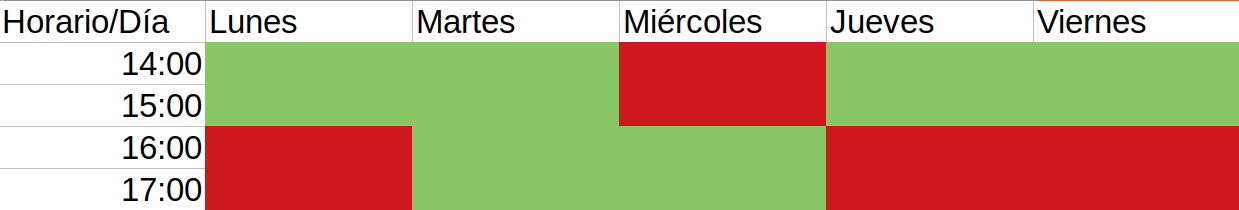
\includegraphics[scale=0.3]{Figures/Asesoria}}
\end{center}
\only<3->{
\includegraphics[scale=0.3]{Figures/HomeroPensando} \hspace{1cm}}
\only<4->{
\includegraphics[scale=0.8]{Figures/Patricio}}
\end{frame}

\subsection{Temas}

\begin{frame}{Temas}
\begin{itemize}
\item<1-20> Introducción
	\begin{itemize}
		\item<2-5> Historia de los computadores. 
		\item<3-5> Modelos de computación. 
		\item<4-5> Partes de los computadores. 
		\item<5> Cuál es el funcionamiento básico de los computadores.
	\end{itemize}
\item<6-20> Introducción a la algoritmia
	\begin{itemize}
		\item<7-11> Representación binaria de la información. 
		\item<8-11> Pseudo-código. 
		\item<9-11> Diagramas de flujo.
		\item<10-11> Variables. 
		\item<11> Condicionales. 
	\end{itemize}
\item<12-20> Introducción a la programación
	\begin{itemize}
		\item<13-19> Elementos principales de Python.
		\item<14-19> Variables y condicionales.
		\item<15-19> Listas y estructura de datos.
		\item<16-19> Iteraciones y ciclos.
		\item<17-19> Escritura y lectura de archivos.
		\item<18-19> Graficación.
		\item<19> Introducción a Pandas y Numpy,
	\end{itemize}
\end{itemize}
\end{frame}

\begin{frame}{Temas}
\begin{center}

\includegraphics[scale=0.6]{Figures/Pregunta}
\end{center}
\end{frame}

\begin{frame}{Sorpresa}
\only<1-> {\Large{\textbf{¡Examen sorpresa!}}}
\only<2-> {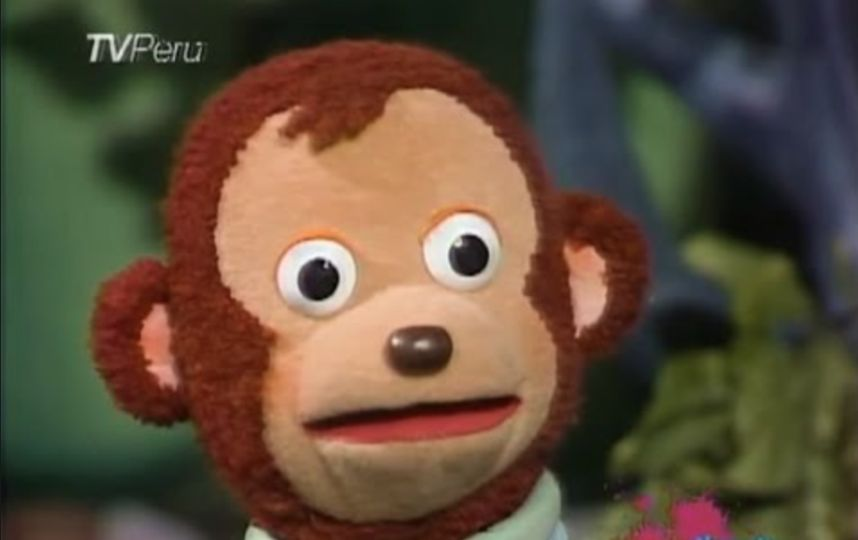
\includegraphics[scale=0.25]{Figures/mono}}
\only<3-> {\Large{\url{https://forms.gle/ZWrufWZDTefGKxsA8}}}
\end{frame}

\subsection{Calificación}
\begin{frame}{Calificación}
\begin{itemize}
\item<1-|alert@1> 3 parciales mensuales del 20\% cada uno.
\item<2-|alert@2> 1 proyecto final del 20\% donde se implemente lo aprendido.
\item<3-|alert@3> Talleres del 20\%.
\end{itemize}
\only<4-> {\Huge{\textcolor{red}{¡Preguntas!}}}
\end{frame}

\begin{frame}
\Huge{Explicación de vídeo}
\end{frame}

\section{Motivación}
\begin{frame}
\begin{center}
\Huge{\textcolor{blue}{Motivación}}
\end{center}
\end{frame}

\begin{frame}{Inicios}
\begin{columns}
\column{.4\textwidth}
\begin{center}
\only<2>{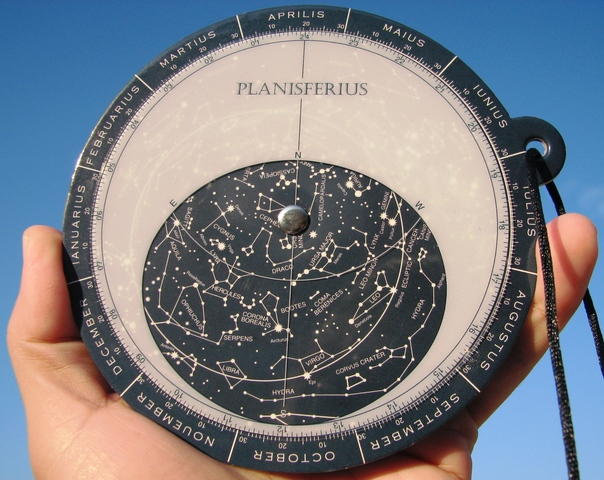
\includegraphics[scale=0.8]{Figures/planis}}
\only<3>{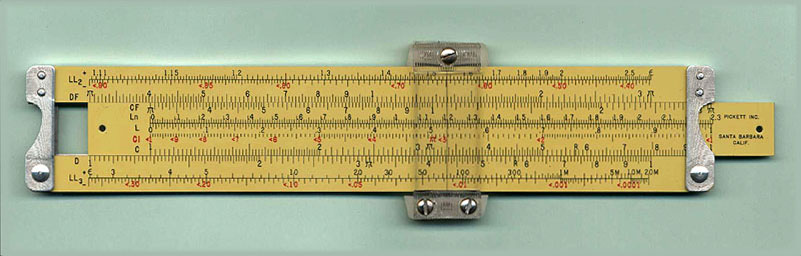
\includegraphics[scale=0.8]{Figures/regla}}
\only<4>{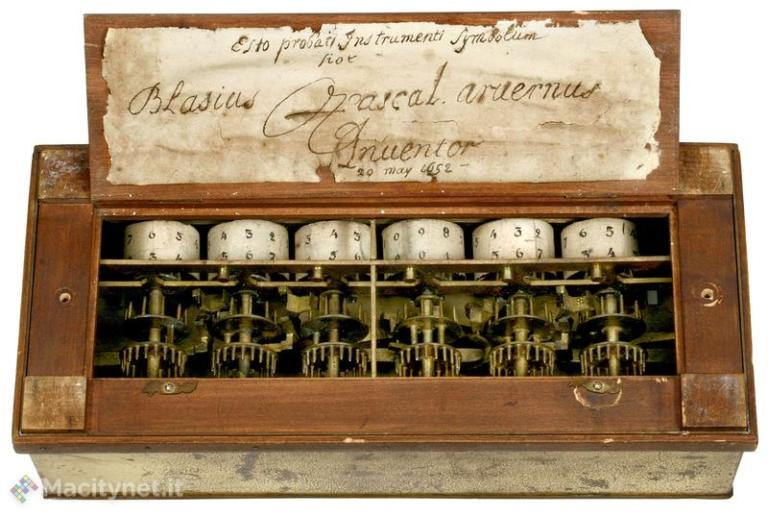
\includegraphics[scale=0.2]{Figures/pascalina}}
\only<5>{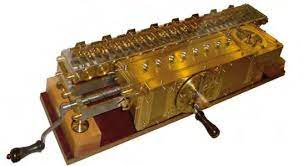
\includegraphics[scale=0.5]{Figures/libniz}}
\end{center}
\column{.4\textwidth}
\only<2-5>{\begin{block}{Eventos} \small 
\begin{itemize}
\item<2- |alert@2> El ábaco, Brújula, Planisferio.
\item<3- |alert@3> 1622: William Oughtred muestra al mundo su regla de calculo. 
\item<4- |alert@4> 1642: Blaise Pascal inventa La pascalina.
\item<5- |alert@5> 1672: Leibnitz mejora la pascalida.
\end{itemize} 
\end{block}}
\end{columns}
\end{frame}

\begin{frame}{Inicios}
\begin{columns}
\column{.4\textwidth}
\begin{center}
\only<1>{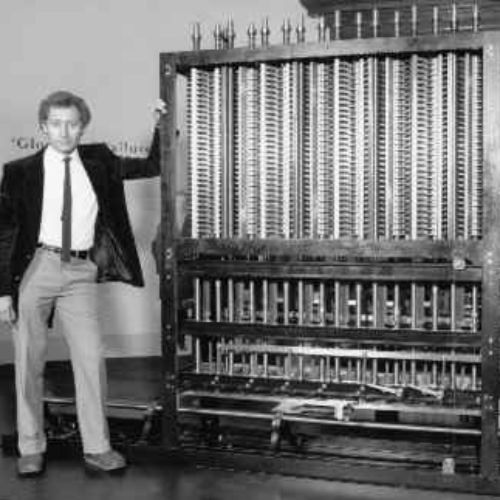
\includegraphics[scale=0.4]{Figures/CharlesBabbage}}
\only<2>{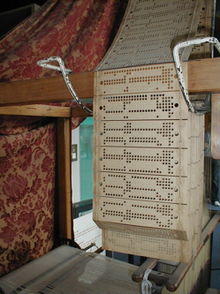
\includegraphics[scale=0.6]{Figures/telares}}
\only<3>{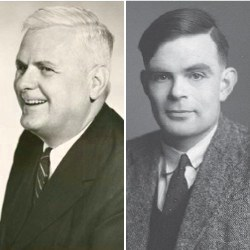
\includegraphics[scale=0.6]{Figures/ChurchTuring}}
\only<4>{
\includegraphics[scale=0.5]{Figures/y-si-era-tan-listo-porque-se-murio}}
\only<5>{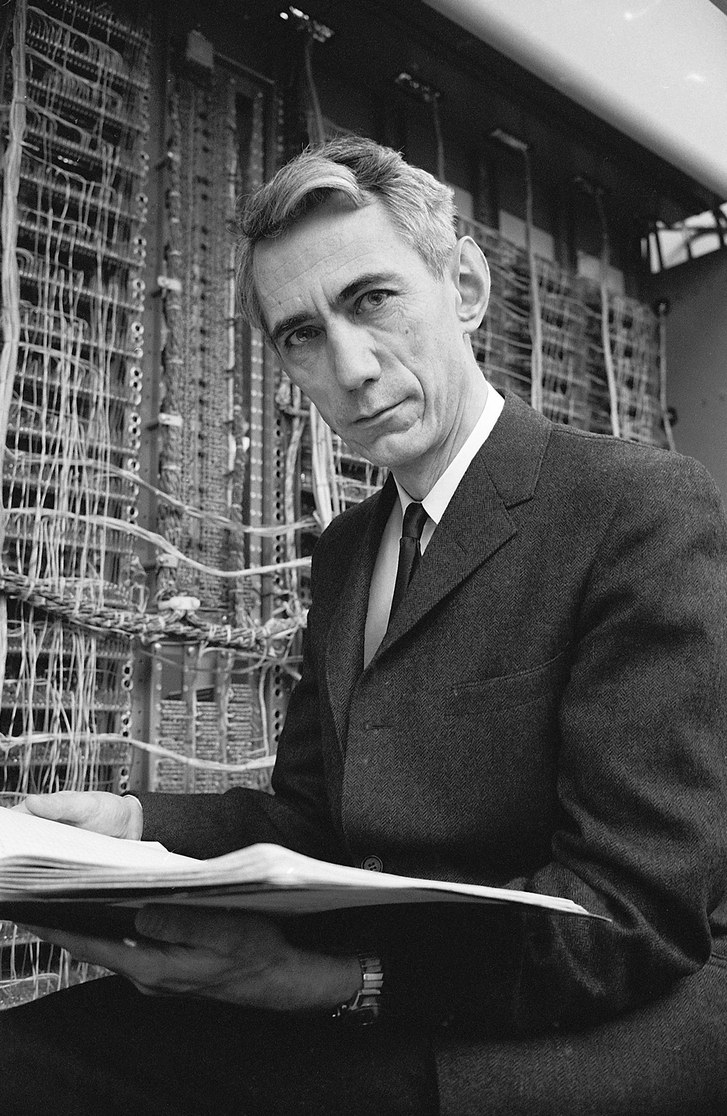
\includegraphics[scale=0.15]{Figures/claude-shannon}}
\end{center}
\column{.4\textwidth}
\only<1-5>{\begin{block}{Eventos} \small 
\begin{itemize}
\item<1- |alert@1> 1833: Charles Babbage crea maquina que suma, resta, multiplica y divide.
\item<2- |alert@2> 1890: Herman Hollerith crea las tarjetas perforadas para maquinas de bordado.
\item<3- |alert@3> 1936: Alan Turing y Alonzo Church:  tesis de Church-Turing 
\item<5- |alert@5> 1938: Claude Shannon: Circuitos de conmutación, Algebra Booleana, Tarjetas perforadas.
\end{itemize} 
\end{block}}
\end{columns}
\end{frame}


\section{Historia de la computación}
\begin{frame}
\begin{center}
\Huge{\textcolor{blue}{Historia de la computación}}
\end{center}
\end{frame}

\begin{frame}
\Huge{\textcolor{blue}{1ra Generación 1938-1956}}
\end{frame}

\begin{frame}{1ra generación}
\begin{center}
Tubos de vacío como circuitos lógicos \pause
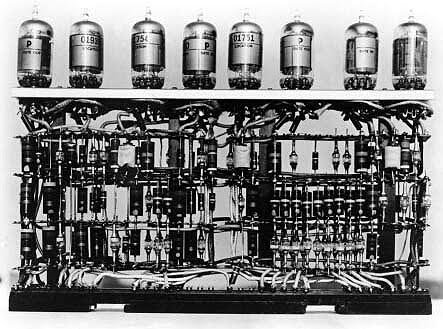
\includegraphics[scale=0.6]{Figures/vtubes}
\end{center}
\end{frame}

\begin{frame}{1ra generación}
\Large{\textcolor{red}{1946: ENIAC (Electronic Numerical Integrator And Computer)}}
\begin{columns}
\column{.4\textwidth}
\begin{center}
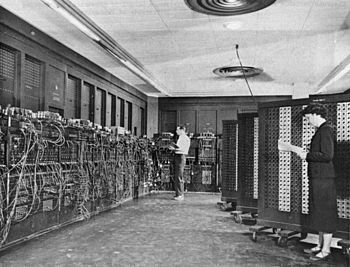
\includegraphics[scale=0.4]{Figures/Eniac}
\end{center}
\column{.5\textwidth}
\only<2-6>{\begin{block}{Caracteristicas} \small 
\begin{itemize}
\item<2- |alert@2> Creada por el grupo de John W. Mauchly y J. Presper Eckert en la universidad de Pensilvania.
\item<3- |alert@3> Construida con 18000 tubos de vacío.
\item<4- |alert@4> Consumía varios kW de potencia eléctrica y pesaba 27 toneladas. 
\item<5- |alert@5> Utilizaba el sistema decimal.
\item<6- |alert@6> Era capaz de efectuar cinco mil sumas por segundo. 
\end{itemize} 
\end{block}}
\end{columns}
\end{frame}

\begin{frame}{1ra generación}
\Large{\textcolor{red}{1949: EDVAC (Electronic Discrete Variable Automatic Computer)}}
\begin{columns}
\column{.4\textwidth}
\begin{center}
\only<2-5>{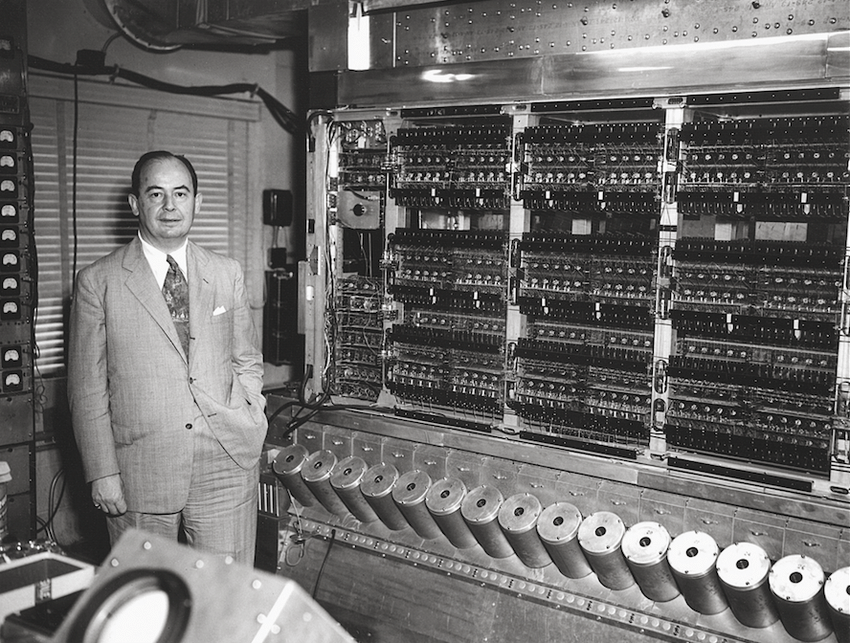
\includegraphics[scale=0.2]{Figures/EDVAC}}
\only<6>{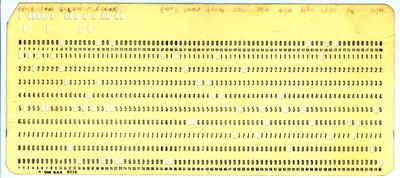
\includegraphics[scale=0.4]{Figures/tarjetaPerf}}
\end{center}
\column{.4\textwidth}
\only<2-6>{\begin{block}{Caracteristicas} \small 
\begin{itemize}
\item<2- |alert@2> Utilizaba el sistema binario.
\item<3- |alert@3> La maquina y los programas estaban separados.
\item<4- |alert@4> Se unio John Von Neumann.
\item<5- |alert@5> 6000 tubos de vacio y 12000 diodos y pesaba 7850 kg.
\item<6- |alert@6> Hacia uso de tarjetas perforadas.
\end{itemize} 
\end{block}}
\end{columns}
\end{frame}

\begin{frame}{1ra generación}
\begin{columns}
\column{.4\textwidth}
\begin{center}
\only<2>{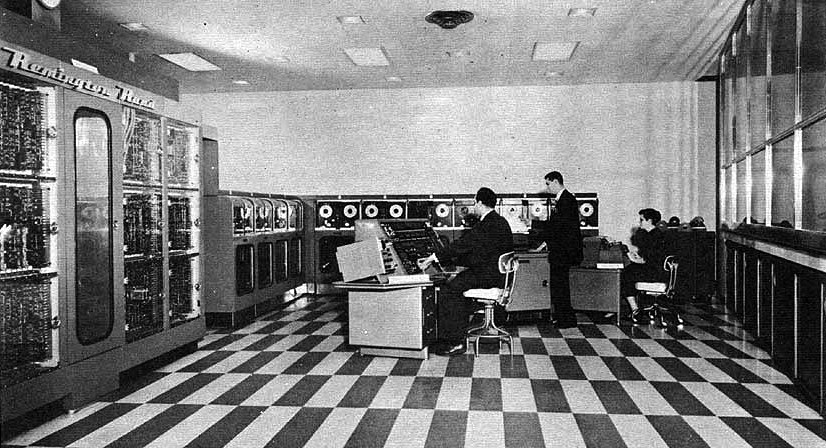
\includegraphics[scale=1.0]{Figures/UNIVAC}}
\only<3>{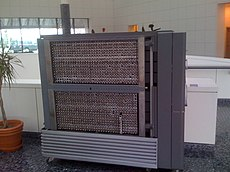
\includegraphics[scale=0.8]{Figures/IBM_701}}
\only<4>{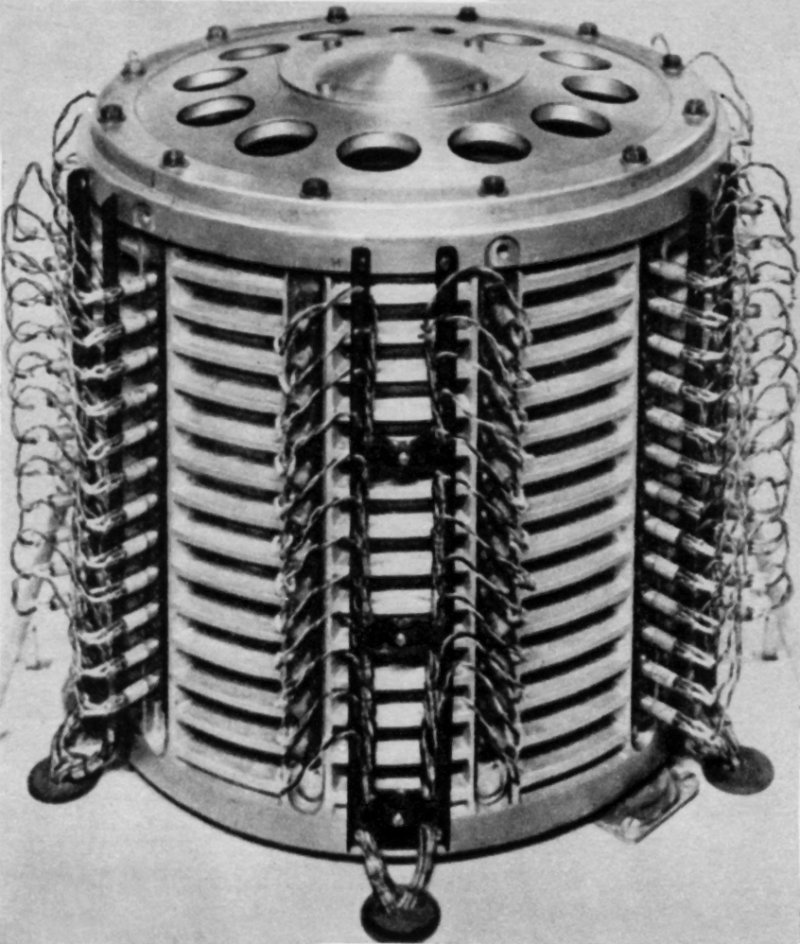
\includegraphics[scale=0.7]{Figures/TamborMag}}
\only<5>{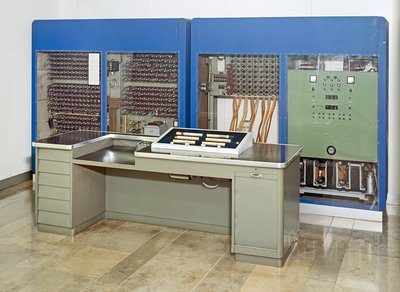
\includegraphics[scale=0.4]{Figures/ZuseZ22}}
\end{center}
\column{.4\textwidth}
\only<2-6>{\begin{block}{Computadoras} \small 
\begin{itemize}
\item<2- |alert@2> 1951: UNIVAC I
\item<3- |alert@3> 1953: IBM 701
\item<4- |alert@4> 1954: Tambor magnetico de IBM
\item<5- |alert@5> 1955: Zuse Z22
\end{itemize} 
\end{block}}
\end{columns}
\end{frame}


\begin{frame}
\begin{center}
\Huge{\textcolor{blue}{2da Generación 1956-1964}}
\end{center}
\end{frame}

\begin{frame}{2da generación}
\begin{center}
Aplicación de los transistores en la computación. \pause
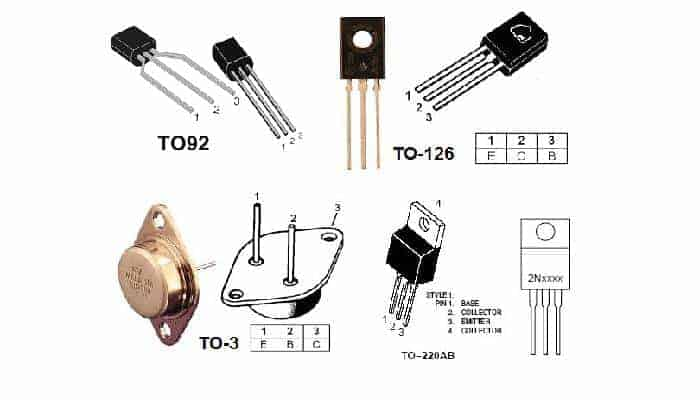
\includegraphics[scale=0.4]{Figures/Transistor}
\end{center}
\end{frame}

\begin{frame}{2da generación}
\begin{columns}
\column{.4\textwidth}
\begin{center}
\only<2>{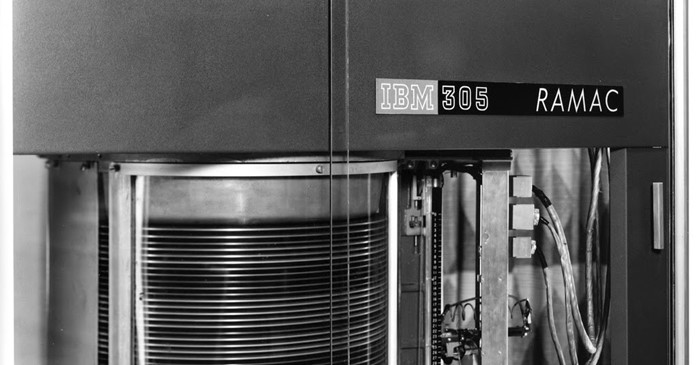
\includegraphics[scale=0.3]{Figures/RAMAC}}
\only<3>{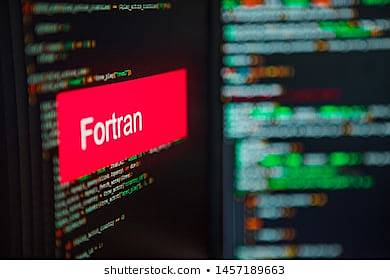
\includegraphics[scale=1.2]{Figures/Fortran}}
\only<4>{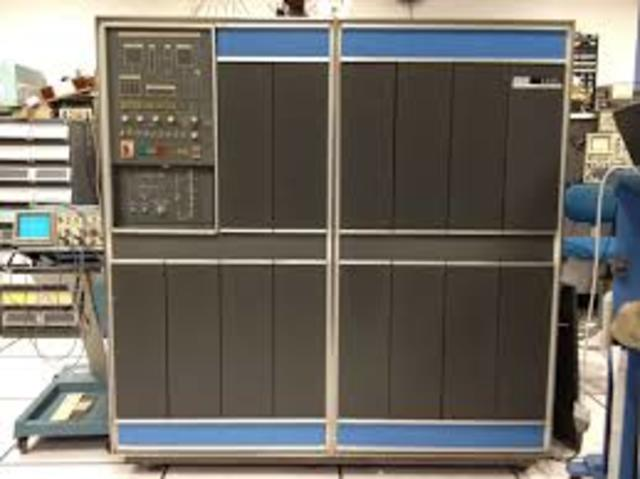
\includegraphics[scale=0.25]{Figures/IBM1401}}
\only<5>{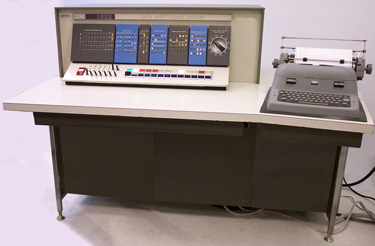
\includegraphics[scale=0.4]{Figures/IBM_1620}}
\only<6>{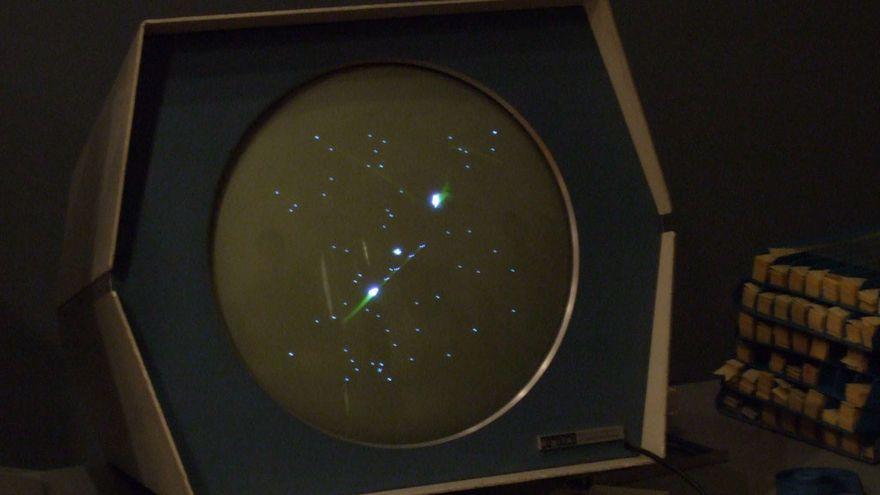
\includegraphics[scale=0.25]{Figures/spacewar}}
\only<7>{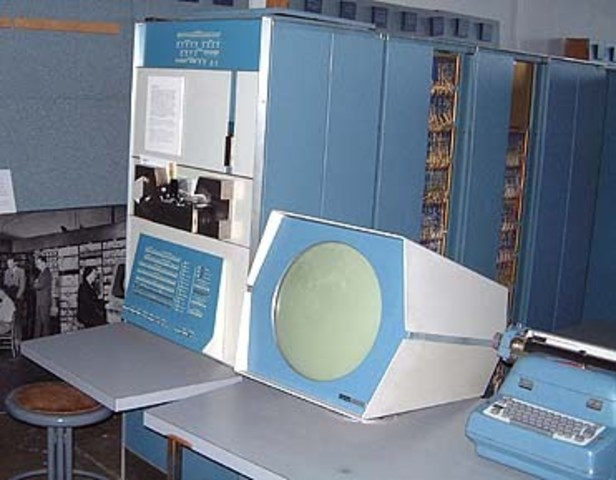
\includegraphics[scale=0.3]{Figures/PDP-1}}
\only<8>{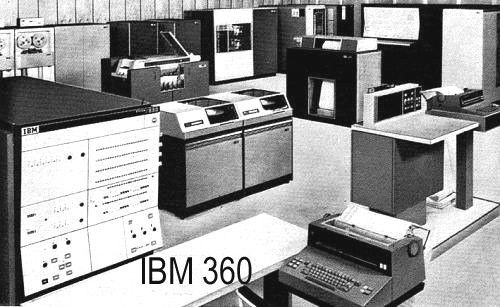
\includegraphics[scale=0.4]{Figures/IBMSerie360}}
\end{center}
\column{.4\textwidth}
\only<2-8>{\begin{block}{Computadoras} \small 
\begin{itemize}
\item<2- |alert@2> 1956: IBM 305 RAMAC
\item<3- |alert@3> 1956: COBOL, FORTRAN
\item<4- |alert@4> 1959: IBM 1401
\item<5- |alert@5> 1960: IBM 1620
\item<6- |alert@6> 1962: Se desarrolla Spacewar!
\item<7- |alert@7> 1962: PDP-1
\item<8- |alert@8> 1964: IBM anuncia la serie 360
\end{itemize} 
\end{block}}
\end{columns}
\end{frame}

\begin{frame}
\Huge{\textcolor{blue}{3ra Generación 1964-1971}}
\end{frame}

\begin{frame}{3ra generación}
\begin{center}
\Huge{¡1964!} \pause aparecen los circuitos integrados. \pause
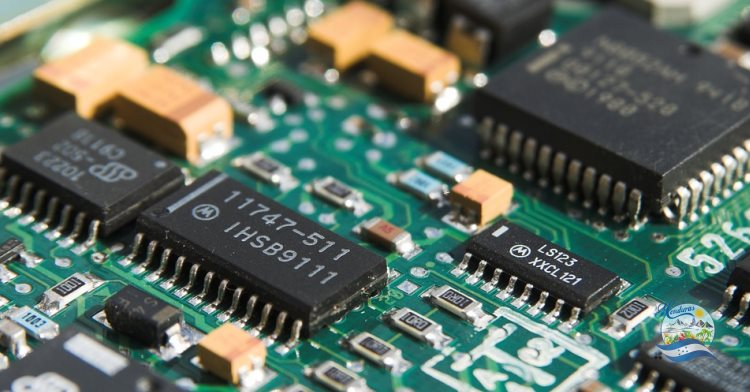
\includegraphics[scale=0.35]{Figures/Circuito_integrado}
\end{center}
\end{frame}

\begin{frame}{3ra generación}
\begin{columns}
\column{.35\textwidth}
\only<2-7>{\begin{block}{Caracteristicas} \small 
\begin{itemize}
\item<2- |alert@2> Menor consumo de energía eléctrica.
\item<3- |alert@3> Aumento de fiabilidad y flexibilidad.
\item<4- |alert@4> Multiprogramación.
\item<5- |alert@5> Renovación de periféricos.
\item<6- |alert@6> Minicomputadoras, no tan costosas y con gran capacidad de procesamiento
\item<7- |alert@7> Se calcula $\pi$ con 500 mil decimales.
\end{itemize} 
\end{block}}
\column{.4\textwidth}
\begin{center}
\only<2>{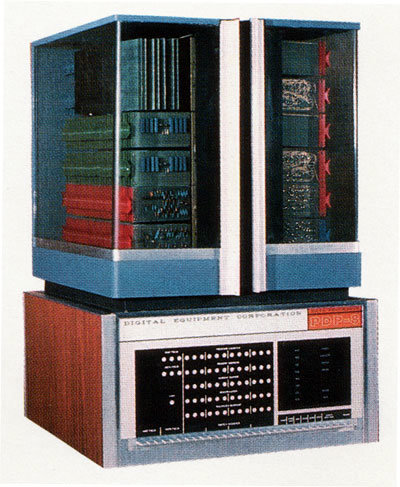
\includegraphics[scale=0.35]{Figures/PDP-8}}
\only<3>{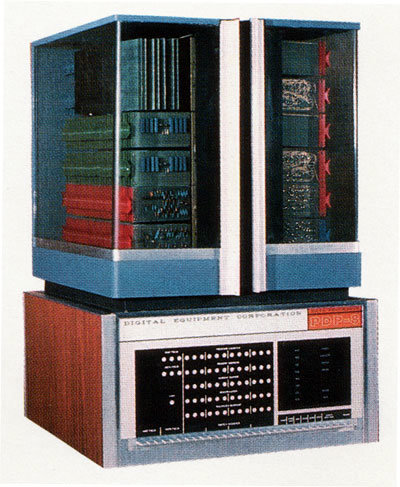
\includegraphics[scale=0.35]{Figures/PDP-8}}
\only<4>{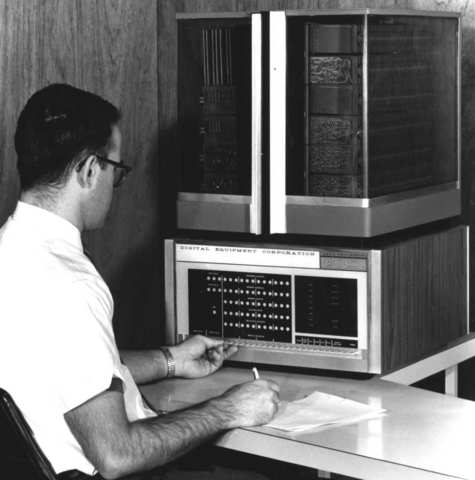
\includegraphics[scale=1.0]{Figures/PDP8-1}}
\only<5>{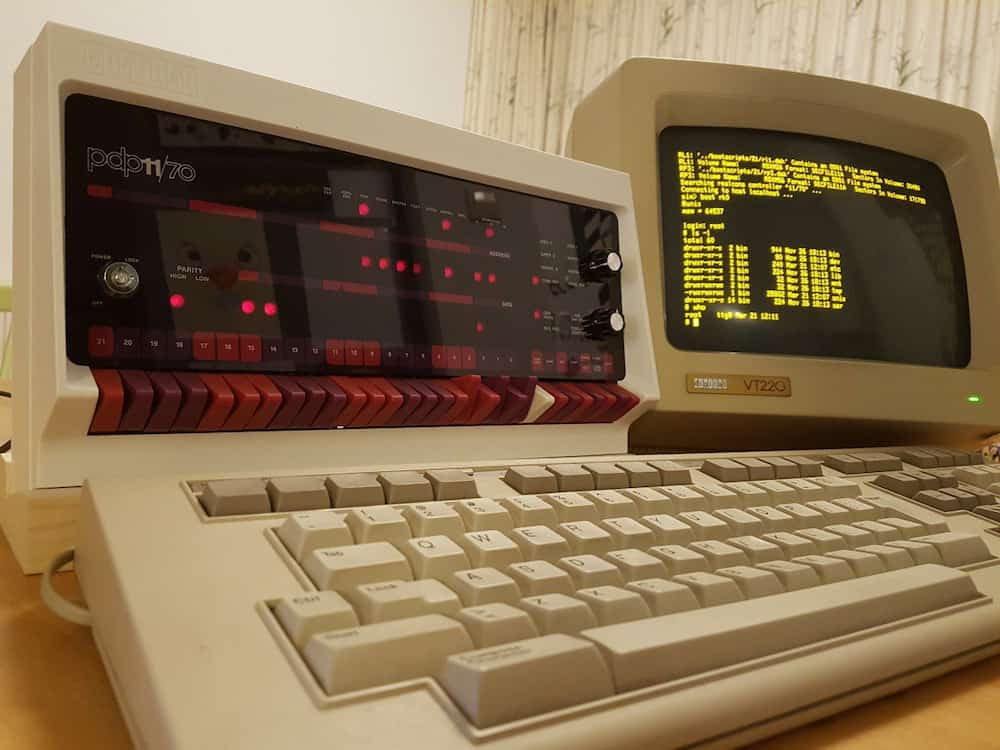
\includegraphics[scale=0.15]{Figures/PiDP-11}}
\only<6>{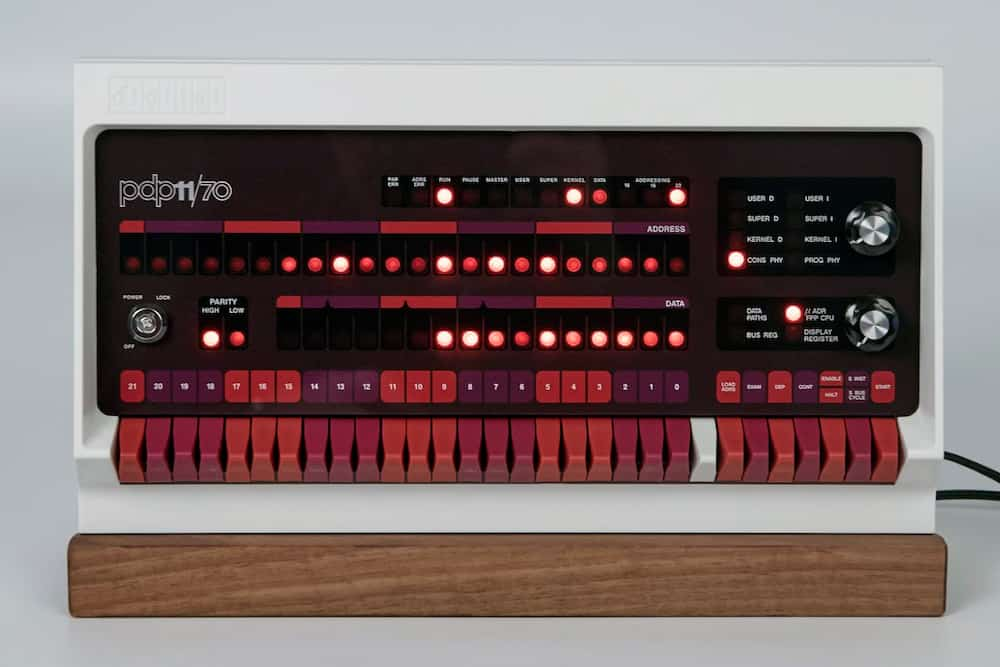
\includegraphics[scale=0.15]{Figures/PiDP11}}
\only<7>{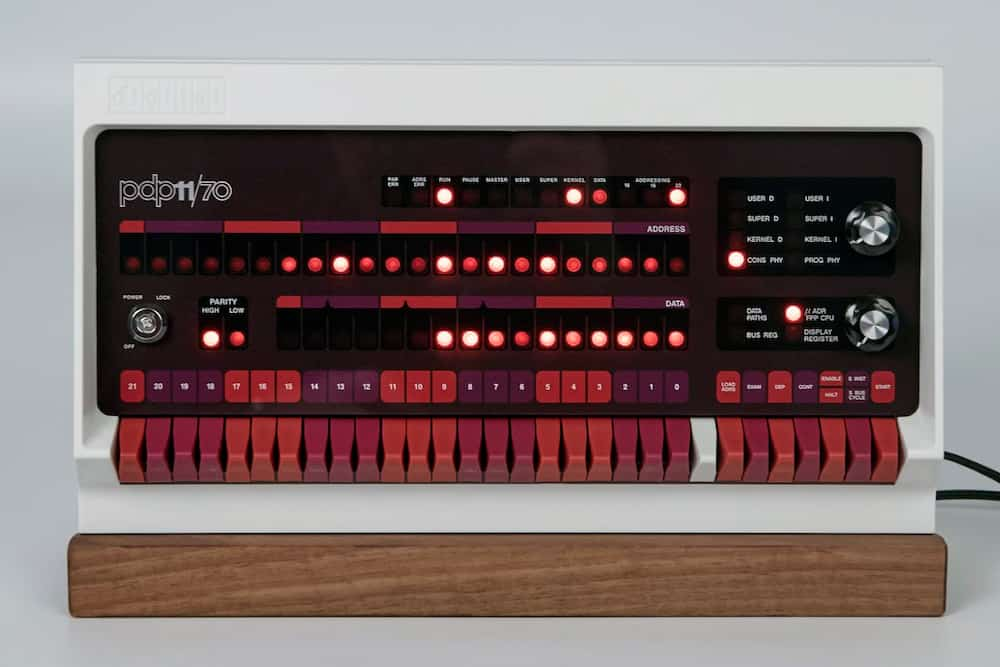
\includegraphics[scale=0.15]{Figures/PiDP11}}
\end{center}
\end{columns}
\end{frame}

\begin{frame}
\Huge{\textcolor{blue}{4ta Generación 1971-1983}}
\end{frame}

\begin{frame}{4ta generación}
\begin{center}
Aparecen los microprocesadores (CPU). \pause
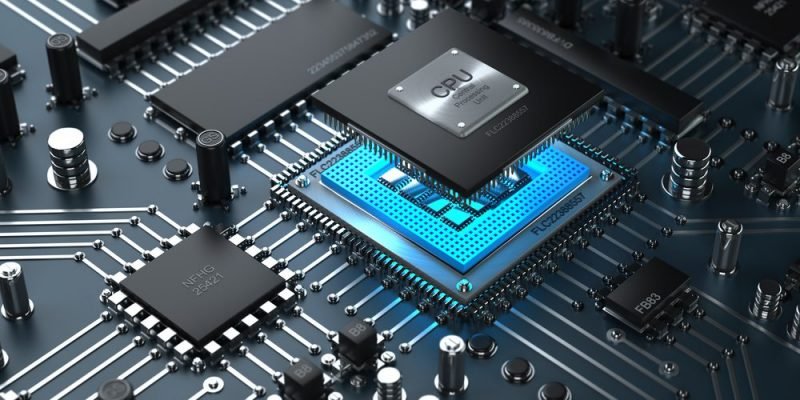
\includegraphics[scale=0.4]{Figures/microprocesador} \pause
La 4ta Generación es el producto de la micro miniaturización de los circuitos electrónicos
\end{center}
\end{frame}

\begin{frame}
\begin{center}
\Huge{\textcolor{red}{Ley de Moore}}
\only<2->{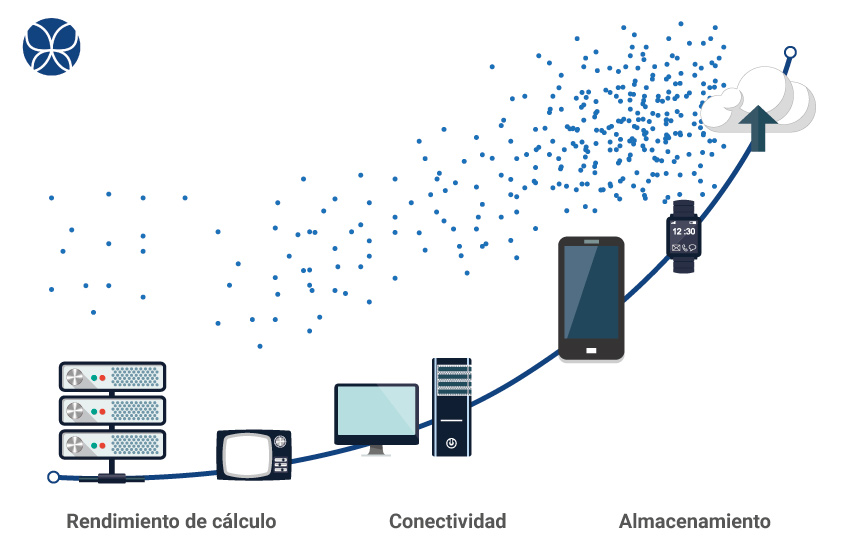
\includegraphics[scale=0.3]{Figures/Ley-de-moore}}
\end{center}
\end{frame}


\begin{frame}{Ley de Moore}
\begin{center}
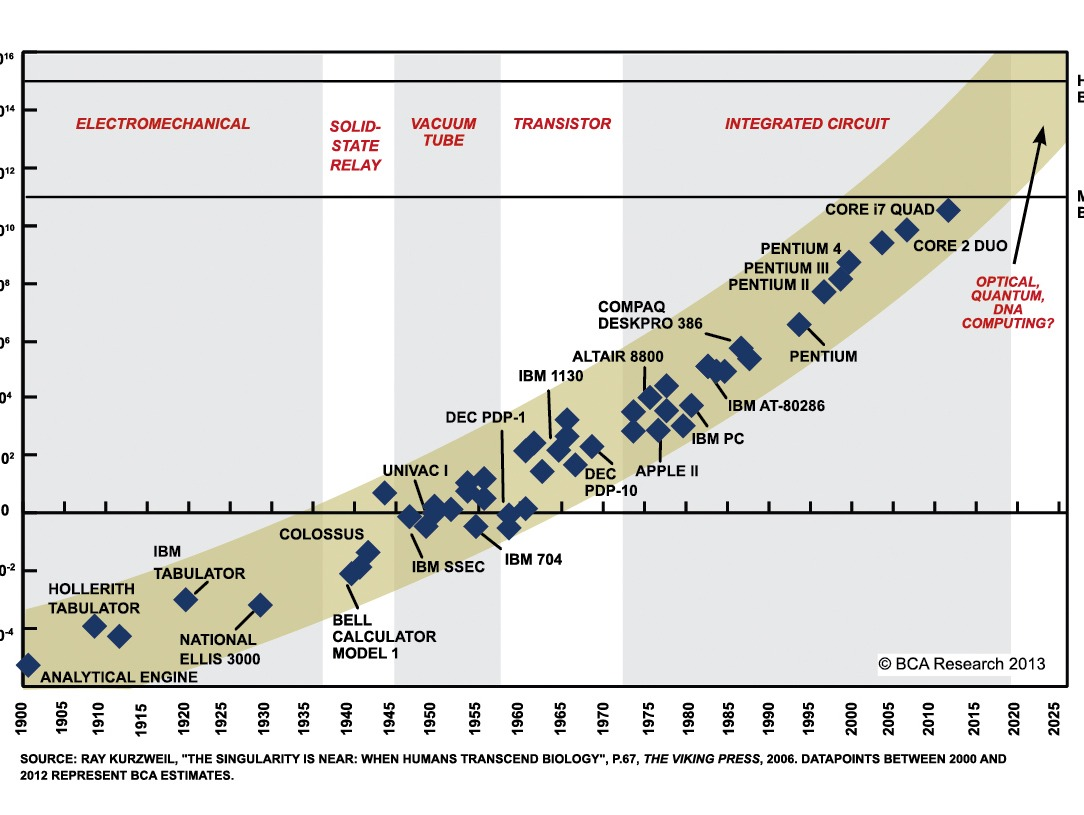
\includegraphics[scale=0.25]{Figures/LeyMoore}
\end{center}
\end{frame}

\begin{frame}{Ley de Moore}
\begin{center}

\includegraphics[scale=0.3]{Figures/desgracia}
\end{center}
\end{frame}


\begin{frame}{4ta generación}
\begin{columns}
\column{.4\textwidth}
\begin{center}
\only<2>{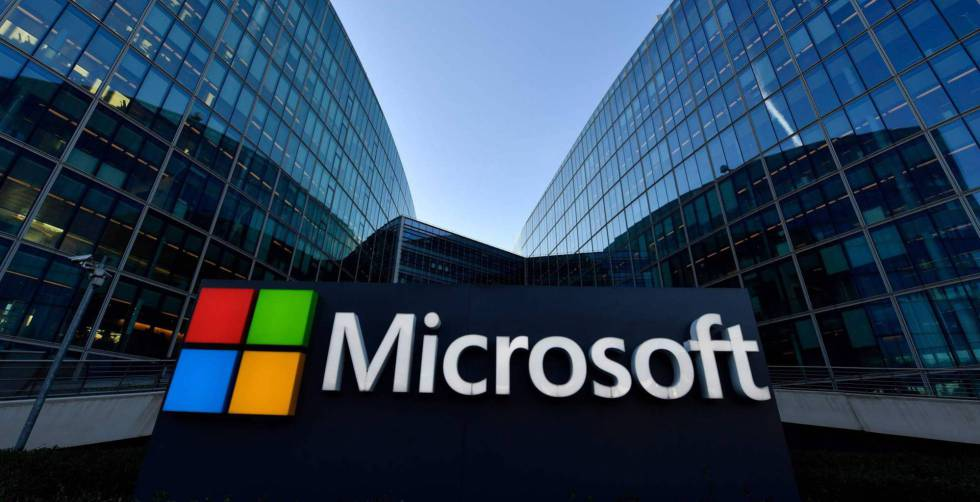
\includegraphics[scale=0.2]{Figures/microsoft}}
\only<3>{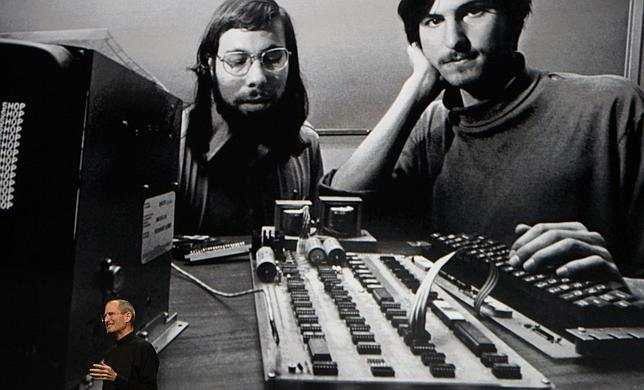
\includegraphics[scale=0.35]{Figures/apple}}
\only<4>{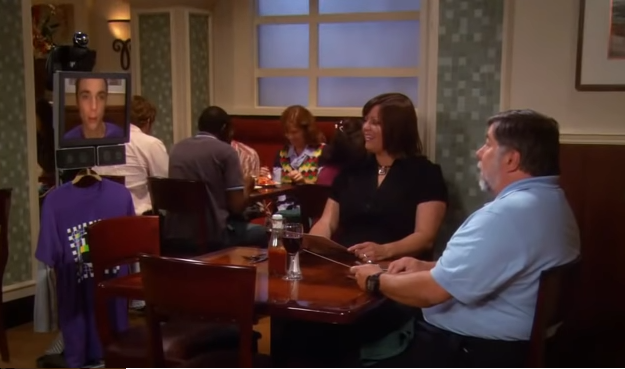
\includegraphics[scale=0.35]{Figures/Shelbot_with_Steve_Wozniak}}
\only<5>{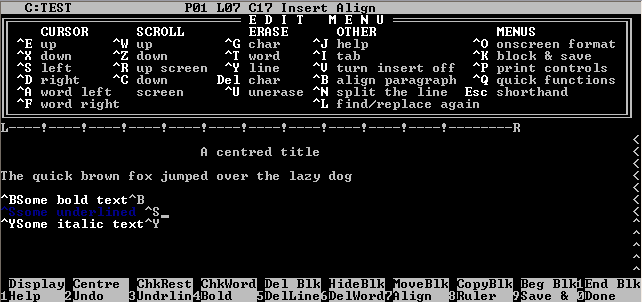
\includegraphics[scale=0.25]{Figures/wordstar}}
\only<6>{
\includegraphics[scale=0.15]{Figures/LisaS}}
\only<7>{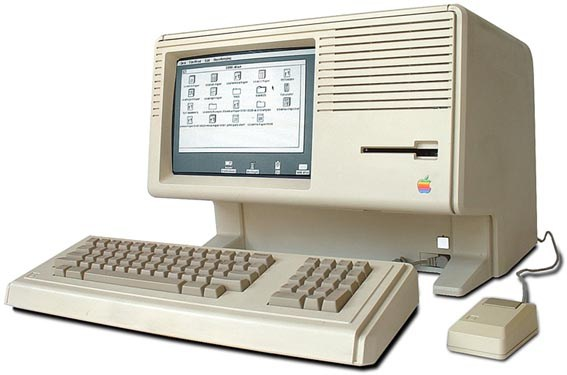
\includegraphics[scale=0.25]{Figures/lisa}}
\only<8>{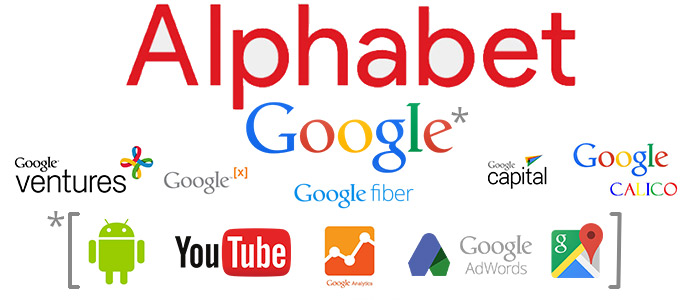
\includegraphics[scale=0.22]{Figures/Google}}
\end{center}
\column{.4\textwidth}
\only<2-8>{\begin{block}{Computadoras} \small 
\begin{itemize}
\item<2- |alert@1> 1975: Inicia Microsoft Corp.
\item<3- |alert@2> 1976: Inicia Apple Computer Corp (Steve Jobs- Steve Wozniak)
\item<5- |alert@3> 1978 Procesadores de texto (WordStar-MicroPro)
\item<6- |alert@4> 1978: Apple presenta LISA, primera computadora con mouse e interfaz grafica. 
\item<8- |alert@5> 1980: Alphabet Inc dueña de Google LLC. 
\end{itemize} 
\end{block}}
\end{columns}
\end{frame}

\begin{frame}
\begin{center}
\includegraphics[scale=0.5]{Figures/theend}
\end{center}
\end{frame}

\begin{frame}
\Huge{\textcolor{blue}{5ta Generación 1983-2022}}
\end{frame}

\begin{frame}{5ta generación}
\begin{itemize}
\item<1- |alert@1> Aparecen computadores de grandes compañias como Epson, HP, ACER, COMPAQ.
\item<2- |alert@2> Comienzan a aparecer los software: Windows 1,0, Juegos, entre otros.
\item<3- |alert@3> 1984: Aparece Machintosh en el mercado, posee mouse y una interfaz gráfica. 
\item<4- |alert@4> Computadoras interconectadas entre sí. Multiprocesamiento en la cpu.
\item<5- |alert@5> 1990: Timothy Jhon Berners-Lee (Tom Berners-Lee) Padre de la World Wide Web. 
\item<6- |alert@6> Monitores planos y tactiles, procesamiento mejorado, portatiles, fibre óptica (mejor velocidad de internet), inteligencia artificial.
\end{itemize}
\begin{center}
\only<3>{\includegraphics[scale=0.3]{Figures/Machintosh}}

\only<5>{Sugiere los términos
HTML (HiperText Markup Language)
HTTP (Hipertext Transfer Protocol)
URL (Uniform Resource Locator) }

\only<6>{Decidir, diseñar y programar APP}
\end{center}
\end{frame}

\begin{frame}
\Huge{\textcolor{blue}{Futuro ...}} \\ \pause
\Large{Se esperan avances en la computación cuántica, inteligencia artificial y otros.}
\end{frame}

\begin{frame}
\begin{center}
\includegraphics[scale=0.7]{Figures/callese}
\end{center}
\end{frame}

{\1
\begin{frame}[plain,noframenumbering]
  \finalpage{“Si he visto más, es poniéndome sobre los hombros de Gigantes”,  Isaac Newton}
\end{frame}}

\end{document}